\documentclass[11pt]{article}
\usepackage{fullpage}
\usepackage{amsthm}
\usepackage{amsmath} 
\usepackage{amssymb}
\usepackage{graphicx}
\usepackage{mathtools}

\graphicspath{ {./imgs/} }

\setlength{\parindent}{0pt}

\title{Information and Coding Theory (CO349) - Coding Theory}
\author{Michael Tsang}

\newtheorem{defn}{Definition}
\newtheorem{eg}{Example}
\newtheorem{theo}{Theorem}
\newtheorem{lem}{Lemma}

\DeclarePairedDelimiter\ceil{\lceil}{\rceil}
\DeclarePairedDelimiter\floor{\lfloor}{\rfloor}

\begin{document}

\maketitle

\section{Error Correcting Codes}
\begin{itemize}
  \item Without loss of generality, a \textbf{message} can be thought of as an integer between $1$ and some parameter $M$.
  \item To transmit a message over a channel, it is encoded using an \textbf{encoder} ($Enc$) associated with a code $C$.
  \item Encoder - any invertible mapping from $[M]$ to $C$, where $[M] = \{ 1, 2, \ldots, M\}$.
  \item Message $x \in [M]$ is encoded to $Enc(x) \in C$.
  \item We assume $\lvert C \rvert = M$.
  \item We use a \textbf{decoder} ($Dec$) to get $x$ back.
  \item $\forall x \in [M] : Dec(Enc(x)) = x$.
\end{itemize}

\subsection{Closest Codeword Decoder}
The \textbf{closest codeword} decoder (\textbf{minimum distance rule}):
\begin{itemize}
  \item Given a received word $y = (y_1, y_2, \ldots, y_n)$, $Dec(y)$ examines every codeword of $C$ and finds the codeword $c = (c_1, c_2, \ldots, c_n)$ that is closest to $y$ in Hamming distance.
  \item $c$ is the error-correction of $y$.
  \item The decoder outputs the (unique) message $x$ that is mapped by the encoder to $c$.
\end{itemize}

This corresponds to the \textbf{maximum likelihood} decoder if the codeword is transmitted over and corrupted by the channel $BSC(p)$.

We expect $BSC(p)$ to corrupt $pn$ transmitted symbols; the actual fraction is concentrated around $pn$.

\textbf{Adversarial channel}: controlled by an ``adversary'' who can see the entire codeword and can corrupt up to $t$ positions, of their choice.
The closest codeword decoder is also the best strategy against adversarial channels.

\subsection{Error Correction up to Half Minimum Distance}
Using closest codeword decoder, any code with minimum distance $d$ can be corrected up to $\ceil*{\frac{d - 1}{2}}$ errors (and in general, no more).

We can therefore say that \textbf{Hamming balls} of radius $\ceil*{\frac{d - 1}{2}}$ around codewords are disjoint:
\[
  B(x, r) := \{ y \in B^n : d_H (x, y) \leq r \}
\]

This reduces the error correction problem to a combinatorial packing problem.

Any code with minimum distance $d$ can \textbf{detect} up to $d - 1$ errors (and in general, no more).
If the received word is valid, then no error, otherwise there has been an error.

\subsection{Erasure Correction}
The channel takes a transmitted sequence and erases some of the symbols, such as in packet networks.

\textbf{Binary erasure channel} ($BEC(p)$): independently at random, erase each bit with probability $p$.

The expected number of erasures is $pn$, and the number of erasures concentrates around $pn$.

\textbf{Adversarial erasure model}: given an ``erasure budget'' of $t$ (say $t = (p + \epsilon)n$), an adversary erases any up to $t$ symbols.

A code with minimum distance $d$ can tolerate any up to $d - 1$ erasures (and in general, no more):
\begin{itemize}
  \item Output any codeword that matches the received pattern. (In the erasure model, symbols which are not erased are correct).
  \item If two codewords match the pattern then they must differ in less than $d$ positions (only up to $d - 1$ can be recovered) which is a contradiction.
\end{itemize}

\section{Linear Codes}
To represent codes, we could list all the codewords, but this would be impractical for large codes.
Instead, we describe an \textbf{encoder} for the code in the form of a \textbf{linear function}.

\begin{itemize}
  \item The encoder interprets $x$ as a vector $(x_1, x_2, \ldots, x_k)$ and multiplies it by a matrix to get the encoding $(y_1, y_2, \ldots, y_n)$.
  \item $(y_1, y_2, \ldots, y_n) = Enc(x_1, x_2, \ldots, x_k) := x \cdot G$, where $G$ is a $k \times n$ (fat) matrix called the generator matrix for the code.
  \item The code can be described by only listing the $kn$ entries of $G$.
\end{itemize}

\subsection{Fields}
A \textbf{field} is a set $F$ equipped with addition and multiplication operations.
It has the required properties/axioms:
\begin{itemize}
  \item $a, b \in F \implies a + b \in F, a \cdot b \in F$ (Closure of addition and multiplication)
  \item $a + (b + c) = (a + b) + c$ (Associativity of addition)
  \item $a \cdot (b \cdot c) = (a \cdot b) \cdot c$ (Associativity of multiplication)
  \item $a + b = b + a$ (Commutativity of addition)
  \item $a \cdot b = b \cdot a$ (Commutativity of multiplication)
  \item $\exists 0 \in F \text{ s.t. } a + 0 = a$ (Neutral element of addition)
  \item $\exists 1 \in F \text{ s.t. } a \cdot 1 = a$(Neutral element of multiplication)
  \item $\forall a \in F, \exists (-a) \in F \text{ s.t. } a + (-a) = 0$ (Additive inverse)
  \item $\forall a \in F \setminus \{ 0 \}, \exists (a^{-1}) \in F \text{ s.t. } a \cdot (a^{-1}) = 1$ (Multiplicative inverse)
  \item $a \cdot (b + c) = (a \cdot b) + (a \cdot c)$ (Distributivity)
\end{itemize}

If F is finite, its \textbf{size} must be a \textbf{power} of a prime: $2, 3, 4, 5, 7, 8, 9, 11, 13 \ldots$

\subsection{Finite Fields}
When $q$ is a prime power, we use the notation $GF(q)$ for the finite field with $q$ elements (sometimes $\mathbb{F}_q$).

\textbf{Prime field}: $\lvert F \rvert$ is \textbf{prime}.

In the prime case, \textbf{modular arithmetic} can be used to realise operations:
\begin{itemize}
  \item $F = \{ 0, 1, 2, \ldots, q - 1 \}$
  \item $a \pm b = (a \pm b) \bmod q$
  \item $a \cdot b = (a \cdot b) \bmod q$
  \item $(a^{-1}) = a^{q - 2} \bmod q$
  \item $\frac{a}{b} = a \cdot (b^{-1})$
\end{itemize}

\subsection{Finite/Galois Field: $GF(q)$}
\begin{itemize}
  \item Finite field with $q$ elements.
  \item From Galois theory, $q$ must be a power of a prime.
  \item When $q$ is even, we always have $x = -x$ and $x + y = x - y$.
  \item When $q = 2$, addition is XOR, multiplication is AND.
  \item Over $GF(2)$, $x_1 + x_2 + \ldots + x_n = 1$ if the number of $1$s is odd, else 0 (parity).
\end{itemize}

Useful:
\begin{align*}
  (a + b) \bmod q = ((a \bmod q) + (b \bmod q)) \bmod q \\
  (a \cdot b) \bmod q = ((a \bmod q) \cdot (b \bmod q)) \bmod q
\end{align*}

\subsection{Linear Codes}
Alphabet $B$ is a finite field $F$ (if alphabet size is a prime power).

The code is the \textbf{row span} of a $k \times n$ generator matrix ($k \leq n$):
\[
  G = 
  \begin{pmatrix}
    c_{11} & c_{12} & c_{13} & \dots  & c_{1n} \\
    c_{21} & c_{22} & c_{23} & \dots  & c_{2n} \\
    \vdots & \vdots & \vdots & \ddots & \vdots \\
    c_{k1} & c_{k2} & c_{k3} & \dots  & c_{kn}
  \end{pmatrix}
\]

That is, $C = \{ x \cdot G : x \in F^k \}$, $Enc(x) = x \cdot G$. 

\begin{itemize}
  \item The rows of $G$ must be \textbf{linearly independent} ($rank(G) = k$), otherwise $Enc$ would not be invertible.
  \item A linear code is the \textbf{left image} of the generator matrix $G$.
  \item The choice of $G$ is not unique, elementary row operations on $G$ do not change the code.
  \item The choice of linear encoder for a linear code is not unique either.
  \item Each row of $G$ must be a codeword.
  \item The zero vector must be a codeword.
  \item If $\overrightarrow{c} and \overrightarrow{c'}$ are codewords, then so are $\overrightarrow{c} + \overrightarrow{c'}$ and $\overrightarrow{c} - \overrightarrow{c'}$.
  \item If $\overrightarrow{c}$ is a codeword, then for any scalar $\lambda \in GF(q), \lambda \cdot \overrightarrow{c}$ must be a codeword.
\end{itemize}

An equivalent definition of a linear code: a \textbf{linear subspace} of $F^n$.
\begin{itemize}
  \item A code $C$ is linear iff $\forall c, c' \in C, \forall \lambda \lambda' \in F : \lambda c + \lambda c' \in C$.
  \item A generator matrix is any matrix whose row span is the code (linear combination of the rows generate all possible codewords).
  \item Rows of $G$ form a \textbf{basis} for the code.
  \item Dimension (message length) of a linear code = $k$.
  \item Size of a linear code over a field of size $q$ is $\lvert C \rvert = q^k$.
  \item Dimension is sometimes extended to non-linear codes as $\log_q(\lvert C \rvert)$, rate is therefore:
    \[
      R(C) = \frac{\log (\lvert C \rvert)}{n (\log q)} = \frac{k (\log q)}{n (\log q)} = \frac{k}{n}
    \]
\end{itemize}

\subsection{Notation: $[n, k, d]$ Codes}
$[n, k, d]$ stands for a linear code of length $n$, generator matrix with $k$ rows, and minimum distance $d$.
To emphasise an alphabet size $q$, we can use the notation $[n, k, d]_q$.

An $[n, k, d]_q$ is thus an $(n, q^k, d)_q$ code because the number of possible messages is $q^k$.

\subsection{Minimum Weight Codewords}
For a vector $c = (c_1, c_2, \ldots, c_n)$ over a field $F$, the \textbf{Hamming weight} is the number of non-zero positions in c:
\[
  wgt(c) := \lvert \{ i \in [n] : c_i \neq 0 \} \rvert
\]

For two codewords $c, c'$:
\[
  d_H(c, c') = wgt(c - c')
\]

For any linear code $C$, minimum distance is equal to the minimum non-zero weight:
\[
  d(C) = \min \{ w > 0 : \exists c \in C \text{ s.t. } wgt(c) = w \}
\]

\subsection{Erasure Correction of Linear Codes}
The codeword $y$ is given by:
\[
  \begin{pmatrix}
    y_1 & y_2 & \dots & y_n
  \end{pmatrix}
  =
  \begin{pmatrix}
    x_1 & x_2 & \dots & x_k
  \end{pmatrix}
  \begin{pmatrix}
    c_{11} & c_{12} & c_{13} & \dots  & c_{1n} \\
    c_{21} & c_{22} & c_{23} & \dots  & c_{2n} \\
    \vdots & \vdots & \vdots & \ddots & \vdots \\
    c_{k1} & c_{k2} & c_{k3} & \dots  & c_{kn}
  \end{pmatrix}
\]

We solve this as a system of linear equations (e.g.\ using Gaussian elimination) to find $x$.
\begin{itemize}
  \item We don't know some of the $y_i$.
  \item If $t$ of the symbols in $y$ are erased, we get a system of $n - t$ linear equations in $k$ unknowns.
  \item Necessary (but not sufficient) to have $t < n - k + 1$.
  \item Sufficient to have $t < d$.
  \item Necessary and sufficient to have rank of the columns that are \textbf{not} erased $= k$.
  \item Corollary 1: $d(C) = 1 + \max \{ t : \text{rank of every } n - t \text{ columns of } G \text{ is } = k\}$.
  \item Corollary 2: $d(C) \leq n - k + 1$, \textbf{singleton bound} for linear codes.
\end{itemize}

\section{Systematic Encoder}
An encoder is \textbf{systematic} if it copies the (entire) message intact somewhere in the codeword.
\begin{itemize}
  \item Through the channel, if no errors or erasures occur then it is trivial to decode.
  \item Errors that do occur are easy to detect: call the encoder and see if a consistent result is obtained with the existing checksum.
\end{itemize}

For a linear code, a systematic encoder corresponds to a generator matrix that contains the $k \times k$ identity matrix as a sub-matrix.
\begin{itemize}
  \item $G$ can be made systematic by Gaussian elimination.
  \item Any linear code has a systematic encoder.
  \item For a set of systematic symbol positions (the $k$ positions among the $n$ codeword symbols where the message is copied), a systematic encoder exists iff the corresponding columns of $G$ are linearly independent.
\end{itemize}

\subsection{MDS Codes}
Some linear codes have the maximal number $\binom{n}{k}$ of systematic encoders, these are \textbf{maximum distance separable} codes.
\begin{itemize}
  \item For an MDS code, every $k \times k$ submatrix of $G$ has rank $k$ (every $k$ columns of G are linearly independent).
  \item Minimum distance of an MDS code is (thus) $n - k + 1$ (singleton bound).
\end{itemize}

Examples include the identity code, repetition code, and parity code.

\subsection{Parity Check Matrix}
Any code can be represented in two ways:
\begin{enumerate}
  \item By the encoder: given a message $x$, what is the encoding of $x$?
  \item By the error detection function: given a received word $(y_1, y_2, \ldots, y_n)$, is it a codeword?
\end{enumerate}

In the case of linear codes, the linear function is specified by a generator matrix: 
\[
  Enc(x) = x \cdot G
\]

Since a linear code is just a $k$-dimensional subspace, the error detection function can always be specified by a system of linear equations (i.e.\ the code is the solution set of a system of linear equations in $n$ unknowns).
For a matrix $H$:
\[
  \mathcal{C} = \{ (c_1, \cdots, c_n) \text{ s.t.\ } H \cdot (c_1, \cdots, c_n)^\intercal = (0, 0, \cdots, 0)^\intercal \}
\]

($\mathcal{C}$ is the linear code).

\begin{itemize}
  \item $H$ is a $r \times n$ matrix over $GF(q)$ which is called a \textbf{parity check matrix} for the code.
  \item The code is the \textbf{right kernel} of $H$, the solution set of the system of $r$ equations in $n$ unknowns ($H \cdot \overrightarrow{c} = \overrightarrow{0}$) specified by $H$.
  \item $r = n - k$ equations are needed, $r$ is called the \textbf{co-dimension}.
  \item Similar to $G$, row operations on $H$ do not change the code.
\end{itemize}

\subsection{Finding a Parity Check Matrix}
When $G$ is in systematic form:
\[
  Enc(x_1, \ldots, x_k) = (x_1, \ldots, x_k, c_{k + 1}, \ldots, c_n)
\]
Given a received word $(y_1, \ldots, y_k, y_{k + 1}, \ldots, y_n)$, compute:
\[
	Enc(y_1, \ldots, y_k) = (y_1, \ldots, y_k, y'_{k + 1}, \ldots, y'_n)
\]
and check whether:
\[
	(y'_{k + 1}, \ldots, y'_n) =  (y_{k + 1}, \ldots, y_n)
\]

In matrix terms, suppose a systematic $G$ is in the form:
\[
  G = 
  \left( \begin{array}{@{}c|c@{}}
     \begin{matrix}
        1 & & & \\
        & 1 & & \\
        & & \ddots & \\
        & & & & 1
     \end{matrix} 
        & A
  \end{array} \right)
\]
for some $k \times (n - k)$ checksum part $A$.
In a non-systematic $G$, $A$ is also what remains after reducing $G$ to systematic form.

Then any codeword $\overrightarrow{c} = (c_1, \ldots, c_n)$ must satisfy $(c_{k + 1}, \ldots, c_n) = (c_1, \ldots, c_k) \cdot A$.

\[
  \left( \begin{array}{@{}c|c@{}}
    A^\intercal &
     \begin{matrix}
        1 & & & \\
        & 1 & & \\
        & & \ddots & \\
        & & & & 1
     \end{matrix} 
  \end{array} \right)
  \begin{pmatrix}
    c_1 \\
    c_2 \\
    \vdots \\
    c_n
  \end{pmatrix}
  =
  \begin{pmatrix}
    0 \\
    0 \\
    \vdots \\
    0
  \end{pmatrix}
\]

\subsection{Minimum Distance and Parity Checks}
Minimum distance $d(C)$ is equal to:
\begin{align*}
  d(C) &= 1 + \max \{ t : \text{every } t \text{ columns of } H \text{ are linearly independent}\} \\
  &= \min\{t : \text{there are } t \text{ linearly dependent columns of } H\}
\end{align*}

This is because if $d(C) = t + 1$, then:
\begin{itemize}
  \item Every $t$ columns of $H$ must be linearly independent, otherwise there would be a non-zero vector $\overrightarrow{c}$ of weight at most $t$ such that $H \cdot \overrightarrow{c} = 0$.
    Then $\overrightarrow{c}$ would be a non-zero codeword of weight less than $d(C)$, a contradiction.
  \item There is a non-zero codeword $\overrightarrow{c}$ of Hamming weight $t + 1$, since $H \cdot \overrightarrow{c} = 0$, this defines a linear dependence between $t + 1$ of the columns of H.
\end{itemize}

\begin{eg}
  What is the best (largest) binary linear code of length $n$ that can \textbf{detect} any one-bit error? ($d(C) \geq 2$)

  Every $2 - 1 = 1$ column of $H$ must be linearly dependent.
  Then every column of $H$ must be non-zero.

  $H$with the smallest number of rows (to make $C$ largest) is:
  \[
    H = 
    \begin{pmatrix}
      1 & 1 & \dots & 1
    \end{pmatrix}
  \]
  The dimension is $k = n - 1$, giving a $[n, n - 1, 2]$ code.
  The parity code is of length $n$.

  (Recall we are using $GF(2)$).
\end{eg}

This leads us to the \textbf{Hamming code}.

\section{Hamming Code}
What is the best (largest) binary code of length $n$ that can \textbf{correct} any one-bit error? ($d(C) \geq 3$)

Every $3 - 1 = 2$ columns of $H$ must be linearly dependent.
Then every column of $H$ must be non-zero and no two columns can be equal.

Suppose $n = 2^r - 1$.

$H$ with the smallest number of rows (to make $C$ largest) is such that the columns enumerate all non-zero $r$-bit strings.

For $n = 7$:
\[
  H =
  \begin{pmatrix}
    0 & 0 & 0 & 1 & 1 & 1 & 1 \\
    0 & 1 & 1 & 0 & 0 & 1 & 1 \\
    1 & 0 & 1 & 0 & 1 & 0 & 1
  \end{pmatrix}
\]

The code is $[7, 4, 3]$.

In general, it is \textbf{$[2^r - 1, 2^r - r - 1, 3]$}.

\subsection{Error Correction of Hamming Codes}
Suppose:
\[
  H =
  \begin{pmatrix}
    0 & 0 & 0 & 1 & 1 & 1 & 1 \\
    0 & 1 & 1 & 0 & 0 & 1 & 1 \\
    1 & 0 & 1 & 0 & 1 & 0 & 1
  \end{pmatrix}
\]

\begin{itemize}
  \item Let $\overrightarrow{c} = x \cdot G$ be the sent codeword.
  \item Recipient receives $\overrightarrow{y} = \overrightarrow{c} + \overrightarrow{e}$, where $\overrightarrow{e}$ is the \textbf{error vector}.
  \item The decoder calculates:
    \begin{align*}
      \overrightarrow{s} &= H \cdot \overrightarrow{y} \\
      &= H \cdot (\overrightarrow{c} + \overrightarrow{e}) \\
      &= H \cdot \overrightarrow{c} + H \cdot \overrightarrow{e} \\
      &= H \cdot \overrightarrow{e} \text{ (as applying $H$ on the codeword is $0$)}
    \end{align*}
  \item If no errors, then $\overrightarrow{s} = \overrightarrow{0}$.
  \item Otherwise, $\overrightarrow{e} = \begin{pmatrix} 0 & 0 & \dots & 1 & \dots & 0 \end{pmatrix}$ (a bit flip), where the $1$ is at the $i$th position.
    \item We can see that $H \cdot \overrightarrow{e} = \overrightarrow{s}$ is the $i$th column of $H$, which is the binary expansion of the integer $i$.
\end{itemize}

\subsection{Syndrome Decoding}
For any linear code with parity check matrix $H$, the \textbf{syndrome} of a received word $\overrightarrow{y}$ is the $(n - k)$-dimensional vector $\overrightarrow{s} = H \cdot \overrightarrow{y}$. \\

If $\overrightarrow{y} = \overrightarrow{c} + \overrightarrow{e}$ for some codeword $\overrightarrow{c}$ and error vector $\overrightarrow{e}$, it is \textbf{always} possible to uniquely identify $\overrightarrow{e}$ (and therefore the correct message $\overrightarrow{c}$), as long as the Hamming weight of $\overrightarrow{e}$ is at most $\floor{\frac{d(C) - 1}{2}}$. \\

\textbf{Proof:}
Suppose there are two distinct $\overrightarrow{e}, \overrightarrow{e'}$, each of weight $\floor{\frac{d(C) - 1}{2}}$, such that $H \cdot \overrightarrow{e} = H \cdot \overrightarrow{e'}$.
Then $H \cdot (\overrightarrow{e} - \overrightarrow{e'}) = 0$, but $(\overrightarrow{e} - \overrightarrow{e'})$ is a non-zero vector of Hamming weight less than $d(C)$, contradiction. 

\subsection{Orthogonality of $G$ and $H$}
Any choice of $G$ and $H$ must be orthogonal:
\[
  G \cdot H^\intercal = 0
\]
That is, the inner product of every row of $G$ and every row of $H$ must be zero.

This is because every row of $G$ is a codeword, then it must satisfy $H$. \\

In linear-algebraic terms, rows of $H$ span the orthogonal space of the code: the orthogonal space of a linear space is the set of vectors that are orthogonal to \textbf{every vector} in the linear space. \\

This orthogonal space is the \textbf{dual code} $\mathcal{C}^\bot$.
The dual of $\mathcal{C}^\bot$ is $\mathcal{C}$.

\subsection{The Dual Code}
If $\mathcal{C}$ is determined by a generator matrix $G$ and parity check matrix $H$, then $\mathcal{C}^\intercal$ is determined by a generator matrix $H$ and a parity check matrix $G$.

\begin{itemize}
  \item The dual code is of length $n$ and dimension $r = n - k$.
  \item The dual code of an MDS code must also be an MDS Code:
    If $\mathcal{C}$ is MDS, then every $k \times k$ submatrix of G must have rank $k$; therefore the minimum distance of $\mathcal{C}^\bot$ must be at least (in fact, exactly) $k + 1 = n - r + 1$; therefore $\mathcal{C}^\bot$ is MDS.
\end{itemize}

\section{Algebraic Codes}
\subsection{Reed-Solomon (RS) Code}
A Reed-Solomon code over $GF(q)$ is determined by a set of \textbf{distinct evaluation points} $\alpha_1, \alpha_2, \ldots, \alpha_n \in GF(q)$.

It is possible to define polynomials over $GF(q)$:
\[
  f(x) = c_0 + c_1x + c_2x^2 + \ldots + c_{k - 1}x^{k - 1}
\]

\begin{itemize}
  \item Given $f$, the \textbf{evaluation vector} of $f(x)$ is:
    \[
      \begin{pmatrix}
        f(\alpha_1) & f(\alpha_2) & \dots & f(\alpha_n)
      \end{pmatrix}
    \]
    \item The codewords of a RS code of dimension $k$ is the set of evaluation vectors of all polynomials of degree $< k$.
    \item It is required that $q \geq n$.
\end{itemize}

The RS code is \textbf{linear}:
\begin{itemize}
  \item Adding two polynomials of degree $< k$ gives a polynomial of degree $< k$.
  \item Multiplying a polynomial of degree $< k$ by a scalar in $GF(q)$ gives a polynomial of degree $< k$.
  \item The code is a \textbf{vector space} and thus linear.
\end{itemize}

\subsection{Reed-Solomon Code: Natural Encoder}
\[
  Enc(b_0, b_1, \ldots, b_{k - 1}) :=
  \begin{pmatrix}
    f(\alpha_1) & f(\alpha_2) & \dots & f(\alpha_n)
  \end{pmatrix}
\]
where $f(x) = b_0 + b_1x + b_2x^2 + \ldots + b_{k - 1}x^{k - 1}$.

The generator matrix for this encoder is the \textbf{Vandermonde matrix}:
\[
  G = 
  \begin{pmatrix}
    1 & 1 & \dots & 1 \\
    \alpha_1 & \alpha_2 & \dots & \alpha_n \\
    \vdots & \vdots & \ddots & \vdots \\
    \alpha_1^{k-1} & \alpha_2^{k-1} & \dots & \alpha_n^{k-1}
  \end{pmatrix}
\]

If $\alpha_1, \alpha_2, \dots, \alpha_n$ are distinct, the rank of the matrix is $k$.

\subsection{Reed-Solomon Code: Minimum Distance}
The weight of $
  \begin{pmatrix}
    f(\alpha_1) & f(\alpha_2) & \dots & f(\alpha_n)
  \end{pmatrix}
$ is at least $n - \lvert \{ \text{roots of $f$ over $GF(q)$} \} \rvert$.
\begin{itemize}
  \item As with real polynomials, a non-zero polynomial $f(x)$ of degree $k - 1$ over $GF(q)$ has less than $k$ roots.
  \item $d(C) \geq n - (k - 1) = n - k + 1$.
  \item Due to the Singleton bound, $d(C) \leq n - k + 1$.
  \item Then it must that $d(C) = n - k + 1$, and the code is thus MDS.
\end{itemize}

A polynomial of degree $\leq d$ can be uniquely interpolated from any set of $d$ known evaluations (e.g.\ given $3$ points, we can find the polynomial of degree $3$).

\subsection{Generalised RS Codes}
Being MDS, a RS code of rate $R$ can correct up to $\frac{1 - R}{2}$ fraction of errors (half the minimum distance).

As RS is MDS, the dual is also MDS.
In fact the dual code is essentially an RS code, it is called a \textbf{generalised RS code}.

\begin{itemize}
  \item A generalised RS code is defined by $\alpha_1, \alpha_2, \dots, \alpha_n \in GF(q)$, and non-zero scalars $\gamma_1, \gamma_2, \ldots, \gamma_n \in GF(q)$, \textbf{not necessarily distinct}.
  \item Codewords are of the form:
    \[
      \begin{pmatrix}
        \gamma_1f(\alpha_1) & \gamma_2f(\alpha_2) & \dots & \gamma_nf(\alpha_n)
      \end{pmatrix}
    \]
  \item This gives the same properties as ordinary RS codes, (where $\gamma_1 = \gamma_2 = \ldots = \gamma_n = 1$).
\end{itemize}

\subsection{Reed-Muller (RM) Codes}
The problem with RS codes is that the alphabet size must be large, at least as large as the desired length.

One solution is going from univariate to \textbf{multivariate polynomials}, giving ($q$-ary) Reed-Muller (RM) codes.

\begin{itemize}
  \item $RM(r, m)$: $m$-\textbf{variate} Reed-Muller code of \textbf{order} $r$.
  \item The codewords are evaluation vectors of polynomials of $m$ variables of degree at most $r$ at \textbf{all points} of $(GF(q))^m$.
\end{itemize}

\subsection{Reed-Muller Code: Degree}
The degree of a polynomial is the maximum degree of its monomials (individual terms):
\[
  \alpha \cdot x_1^{d_1} \cdot x_2^{d_2} \cdot \ldots \cdot x_m^{d_m} \text{ has degree }
  d_1 + d_2 + \ldots + d_m
\]
where $x_i$ are distinct variables.

\subsection{Reed-Muller Code: Encoder}
The standard encoder of $RM(r, m)$ interprets the message as a coefficient vector of a polynomial in $m$ variables and degree at most $r$, outputting the vector consisting of evaluations of these polynomials at all points of $(GF(q))^m$.
\begin{eg}
  For $RM(2, 3)$:
  \[
    Enc(b_0, \ldots, b_9) = (\text{evaluations of } f(x, y, z) \text{ everywhere})
  \]
  where
  \[
    f(x, y, z) = b_0 + b_1x + b_2y + b_3z + b_4x^2 + b_5y^2 +b_6z^2 + b_7xy + b_8xz + b_9yz
  \]

  Dimension $k = 10$, length $n = q^3$.
\end{eg}

\begin{itemize}
  \item The alphabet size can be as small as $2$.
  \item In general, the length is $n = q^m$ as we evaluate $f$ everywhere.
  \item The dimension is $k = \binom{m + r}{m} = \binom{m + r}{r}$.
\end{itemize}

The dimension is the number of monomials of polynomial $f(x_1, \ldots, x_m)$ of degree at most $r$.
To find $k$, we want the number of combinations of non-negative integers $d_1, d_2, \ldots, d_m$ such that $d_1 + d_2 + \ldots + d_m \leq r$, which is $k = \binom{m + r}{m}$.
This is only valid if $q > r$, otherwise we may count some monomials several times.

\subsection{Minimum Distance of $RM(r, m)$}
\textbf{Schwartz-Zippel Lemma} states that any polynomial (possibly multivariate) of degree at most $r$, is zero on at most $\frac{r}{q}$ fraction of all possible points.

Then the minimum distance of $RM(r, m)$ is:
\[
  \min \{ \text{Hamming weight of codewords}\} = \min \{ n - \text{ number of zeroes}\} \geq q^m - rq^{m-1}
\]
(This is non-trivial only when $r < q$).

The relative distance (the minimum distance divided by length) of $RM(r, m)$ is:
\[
  \geq (q - \frac{r}{q})
\]

An important special case is $r = 1$.

\subsection{First Order Reed-Muller Codes}
Special case when $q = 2$ and $r = 1$, also know as the \textbf{Hadamard Code}.
\begin{itemize}
  \item Length: $n = 2^m$.
  \item Dimension: $k = \binom{m + r}{r} = m + 1$.
  \item Distance $\geq n\left(1 - \frac{r}{q}\right) = 2^{m - 1}$ (actually exact).
\end{itemize}

The encoder:
\[
  Enc(a_0, \ldots, a_m) = (f(0, 0, \ldots, 0), \ldots, f(1, 1, \ldots, 1))
\]
where
\[
  f(x_1, \ldots, x_m) := a_0 + a_1x_1 + \ldots + a_mx_m
\]

In general, the first order RM code is the dual of extended Hamming code.
This gives it amazing error tolerance but it quickly becomes inefficient.

\section{How Good can a Code be?}
\begin{itemize}
  \item $A(n, d)$: maximum possible size of a binary code of length $n$, minimum distance $/geq d$.
  \item $A_q(n, d)$: same, over $q$-ary alphabet.
  \item In general, we do not know much about the exact values of these.
  \item We know that increasing $d$ decreases $A$, and increasing $n$ or $q$ increases $A$.
  \item We fix $q$ (say $q = 2$), omit $n$, and look at the asymptotic situation:
    \[
      R_q(\delta) := \limsup_{n \rightarrow \infty} \frac{\log_q A_q(n, \floor{\delta n})}{n}
    \]
  \item We find the maximum possible \textbf{rate} for a given \textbf{relative distance} $\delta$.
\end{itemize}


\begin{figure}[h]
  \caption{Graph of the rate.}
  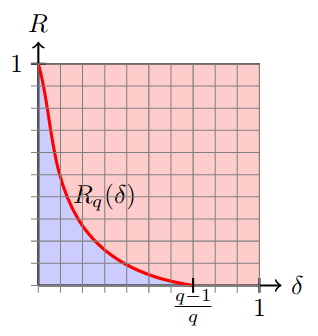
\includegraphics[scale=0.4]{rategraph}
  \centering
\end{figure}

\begin{itemize}
  \item The pink region is impossible, the blue region is possible.
  \item We know the Singleton bound:
    \[
      k \leq n - d + 1
    \]
  \item We divide by $n$, and making $n$ tend to infinity:
    \[
      R_q(\delta) \leq 1 - \delta
    \]
  \item For a fixed $q$, better bounds are known.
  \item \textbf{Plotkin bound}:
    \begin{itemize}
      \item If $\delta \geq \frac{q - 1}{q}$, $R_q(\delta) = 0$.
      \item Else, $R_q(\delta) \leq 1 - \frac{\delta q}{q - 1}$.
    \end{itemize}
\end{itemize}

\subsection{Major Known Bounds for $q = 2$}
\begin{figure}[h]
  \caption{Known bounds.}
  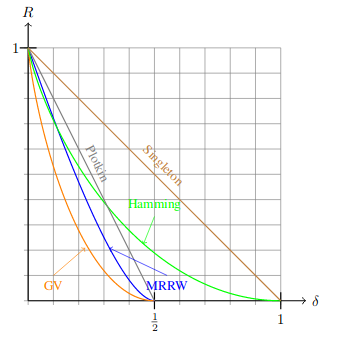
\includegraphics[scale=0.4]{bounds}
  \centering
\end{figure}

Upper bounds on $R_q(\delta)$:
\begin{itemize}
    \item Singleton, Plotkin, Hamming, MRRW.
    \item \textbf{Hamming (or Sphere packing/Packing) bound}:
      \[
        R_q(\delta) \leq 1 - h_q\left(\frac{\delta}{2}\right)
      \]
    \item \textbf{MRRW}:
      \[
        R_q(\delta) \leq h\left(\frac{1}{2} - \sqrt{\delta (1 - \delta)}\right)
      \]
\end{itemize}

Lower bound on $R_q(\delta)$:
\begin{itemize}
  \item \textbf{GV (Gilbert-Varshamov Bound)}:
    \[
      R_q(\delta) \geq 1 - h_q(\delta)
    \]
\end{itemize}

The $q$-ary entropy function:
\[
  h_q(x) := -x\log_q(x) - (1 - x)\log_q(1 - x) + x\log_q(q - 1)
\]

The binary entropy function:
\[
  h(x) := -x\log_2(x) - (1 - x)\log_2(1 - x)
\]

\section{Hamming Bound}
Recall the Hamming ball:
\[
  B(x, r) := \{ y \in (GF(q))^n : d_H(x, y) \leq r \}
\]

In any $(n, M, d)$ code, Hamming balls of radius $r = \floor{\frac{d - 1}{2}}$ centered around the $M$ codewords must not collide.

We can say that each codeword $c$ eats up (at least) $\lvert B(c, r) \rvert$ points in the space $(GF(q))^n$ that cannot be assigned to any other codewords.
This volume does not depend on the center $c$.

Then $Vol_q(n, r)$ is the volume of an $n$-dimensional Hamming ball at radius $r$ over alphabet size $q$.

Any $(n, M, d)_q$ code must satisfy:
\[
  M \leq \frac{q^n}{Vol_q(n, r)}
\]
Taking $\log$ from both sides:
\[
  k \leq n - \log_q(Vol_q(n, r))
\]

Then the \textbf{Hamming bound} for any $(n, M, d)_q$ code is:
\[
  \frac{k}{n} \leq 1 - \log_q\left(Vol_q \left(n, \floor{\frac{d - 1}{2}}\right)\right) / n
\]

\subsection{Hamming Bound: $Vol_q{n, r}$}
\[
  Vol_q(n, r) = 1 + (q - 1)\binom{n}{1} + (q - 1)^2 \binom{n}{2} + \ldots + (q - 1)^r \binom{n}{r}
\]

\begin{itemize}
  \item When $q = 2$:
    \[
      Vol(n, r) = \sum_{i = 0}^r \binom{n}{r}
    \]
  \item Recall:
    \[
      \binom{n}{i} = \frac{n!}{i!(n - i)!}
    \]
  \item \textbf{Stirling's approximation}:
    \[
      n! \approx \sqrt{2\pi n}\binom{n}{e}^n
    \]
  \item Useful to know:
    \[
      \binom{n}{i}^i \leq \binom{n}{i} \leq \binom{ne}{i}^i
    \]
  \item Then, when $r$ is constant, we have $Vol(n, r) = O(n^r)$.
\end{itemize}

\subsection{Hamming Bound: Stirling's Approximation}
Using Stirling's Approximation and assuming $r \leq \frac{q - 1}{q}$:
\[
  q^{nh_q \left(\frac{r}{n}\right) - o(n)} \leq Vol_q(n, r) \leq q^{nh_q \left(\frac{r}{n}\right)}
\]
Which means:
\[
  \frac{\log_q(Vol_q(n, r))}{n} \geq h_q \left(\frac{r}{n}\right) - o(1)
\]
Recalling $o(1)$ meaning that something tends to $0$ as $n$ grows.

Plugging in the Hamming bound, when $d := \delta n$:
\[
  \frac{k}{n} \leq 1 - \log_q\left(Vol_q \left(n, \floor{\frac{d - 1}{2}}\right)\right) / n
  \leq 1 - h_q \left(\frac{\delta}{2}\right) + o(1)
\]

If we tend $n$ to infinity:
\[
  R_q(\delta) \leq 1 - h_q \left(\frac{\delta}{2}\right)
\]

\section{Gilbert-Varshamov (GV) Bound}
A simple greedy algorithm to construct a non-linear $(n, M, d)_q$ code:
\begin{enumerate}
  \item Start with the whole space $S := (GF(q))^n$ and the empty code $C$.
  \item Pick any $c \in S$ and add $c$ as a codeword to $C$.
  \item Remove the Hamming ball of radius $d - 1$ around $c$ from $S$.
  \item Go back to step $2$ if $S \neq \emptyset$.
\end{enumerate}

This gives a code with minimum distance at least $d$.

Each codeword added to $C$ eats up at most $Vol_q(n, d - 1)$ of the space.

The number of steps until the algorithm runs out of codewords to add is at least $\frac{q^n}{Vol_q(n, d - 1)}$.

\[
  M \geq \frac{q^n}{Vol_q(n, d - 1)}
\]
\[
  \text{rate } = \frac{\log_q(M)}{n} \geq \frac{n - \log_q(Vol_q(n, d - 1))}{n} \geq 1 - h_q \left(\frac{d - 1}{n}\right)
\]

If $d = \delta n$ and $n \rightarrow \infty$, then $R_q(\delta) \geq 1 - h_q(\delta)$.

\subsection{Hamming vs.\ Gilbert-Varshamov}:
\[
  1 - h_q(\delta) \leq R_q(\delta) \leq 1 - h_q \left(\frac{\delta}{2}\right)
\]

\subsection{GV Bound for Linear Codes}
Most linear codes achieve the GV bound.

We count how many codes there are, and for a given parameter $d$ split into sets containing codes that contain a non-zero codeword of weight $< d$ (call them the \textbf{bad codes}), and those which do not.

The number of codes is much more than the number of bad codes.

\subsection{Valid Generator Matrices}
The number of valid $k \times n$ generator matrices is:
\begin{align*}
  (q^n - 1)(q^n - q)(q^n - q^2) \ldots (q^n - q^{k - 1})
  &= q^{nk} \left(1 - \frac{1}{q^n}\right)\left(1 - \frac{1}{q^{n - 1}}\right)\left(1 - \frac{1}{q^{n - 1}}\right)\ldots\left(1 - \frac{1}{q^{n - k + 1}}\right) \\
  &\geq q^{nk}\left(1 - \frac{1}{q^n}\right)\left(1 - \frac{1}{q^{n - 1}}\right)\left(1 - \frac{1}{q^{n - 2}}\right)\ldots\left(1 - \frac{1}{q^2}\right) \\
  &\geq q^{nk} \left(1 - \frac{1}{q^n} - \frac{1}{q^{n - 1} - \ldots - \frac{1}{q^2}}\right) \\
  &\geq q^{nk} \left(1 - \frac{1}{q^2 - 1}\right) \\
  &> \frac{1}{2}q^{nk}
\end{align*}

It then follows that more than half of the $q^{n(n - k)}$ choices of an $(n - k) \times n$ matrix $H$ are valid parity matrices of length $n$, dimension $k$.

\subsection{Codes containing $c$}
The number of linear codes of dimension $k$ that can contain $c$ as a codeword is at most $q^{(n - k)n - (n - k)}$.
This is equivalent to the number of parity check matrices which satisfy $H \cdot c = \overrightarrow{0}$, which we can get from recalling that $c$ defines a linear dependence on the columns of $H$, which determines one column of $H$ given the rest of $H$.

The fraction of all possible choices of $H$ (valid or not) corresponding to the codes containing $c$ is at most $\frac{1}{q^{n - k}}$.

\subsection{Codes containing a codeword of weight $< d$}
We know that it is at most $\frac{Vol_q(n, d)}{q^{n - k}}$.

We are therefore left with a code of distance at least $d$, provided that:
\begin{align*}
  \frac{Vol_q(n, d)}{q^{n - k}} &< \frac{1}{2} \\
  \frac{q^{nh_q\left(\frac{d}{n}\right)}}{q^{n - k}} &< \frac{1}{2}
\end{align*}

Let $d = \delta n, R = \frac{k}{n}$, it suffices to have:
\[
  \frac{1}{q^{n(1 - R - h_q(\delta))}} < \frac{1}{2}
\]

If $n$ is large, this means it suffices to have $R < 1 - h_q(\delta)$.
This is the GV bound.

\end{document}
